% =============================================================================
% P1 --- version revisada: GradCAM como evidencia de que la clasificacion
% global NO se apoya en la morfologia de las rafagas.
% Sustituye integramente la seccion P1 del capitulo 5.
% Figuras nuevas: resnet18_gradcam_drone.png y resnet18_gradcam_interference.png
% (versiones de dos columnas: Entrada | GradCAM de la clase verdadera).
% =============================================================================

\section{P1 --- ¿Es reconocible la firma OcuSync mediante clasificación global?}
\label{sec:bloque_resnet_detector}

\subsection{Planteamiento del experimento}
\label{sec:p1_planteamiento}

La primera aproximación al problema consiste en entrenar un clasificador binario ResNet18 sobre el espectrograma completo para asignar la etiqueta \emph{drone} o \emph{interference} a cada imagen. Esta formulación evita la complejidad del etiquetado regional: basta con la etiqueta de la captura de la que procede cada espectrograma.

Se parte de una ResNet18 preentrenada en ImageNet, congelando las primeras tres capas y sustituyendo la cabeza de clasificación original por una capa \texttt{Linear(512,~2)}. El modelo se entrena durante \num{20}~épocas con el optimizador AdamW (tasa de aprendizaje \num{1e-4}, \emph{weight decay} \num{1e-4}), planificador \texttt{CosineAnnealingLR} y tamaño de lote \num{32}. Se aplica la normalización frecuencial \texttt{FrequencyNormalize} y la semilla se fija en 42.

\subsection{Resultados}
\label{sec:p1_resultados}

La \cref{fig:resnet18_binary_curvas} muestra la evolución de la pérdida y el F1~macro en entrenamiento y validación a lo largo de las veinte épocas.

\begin{figure}[htbp]
    \centering
    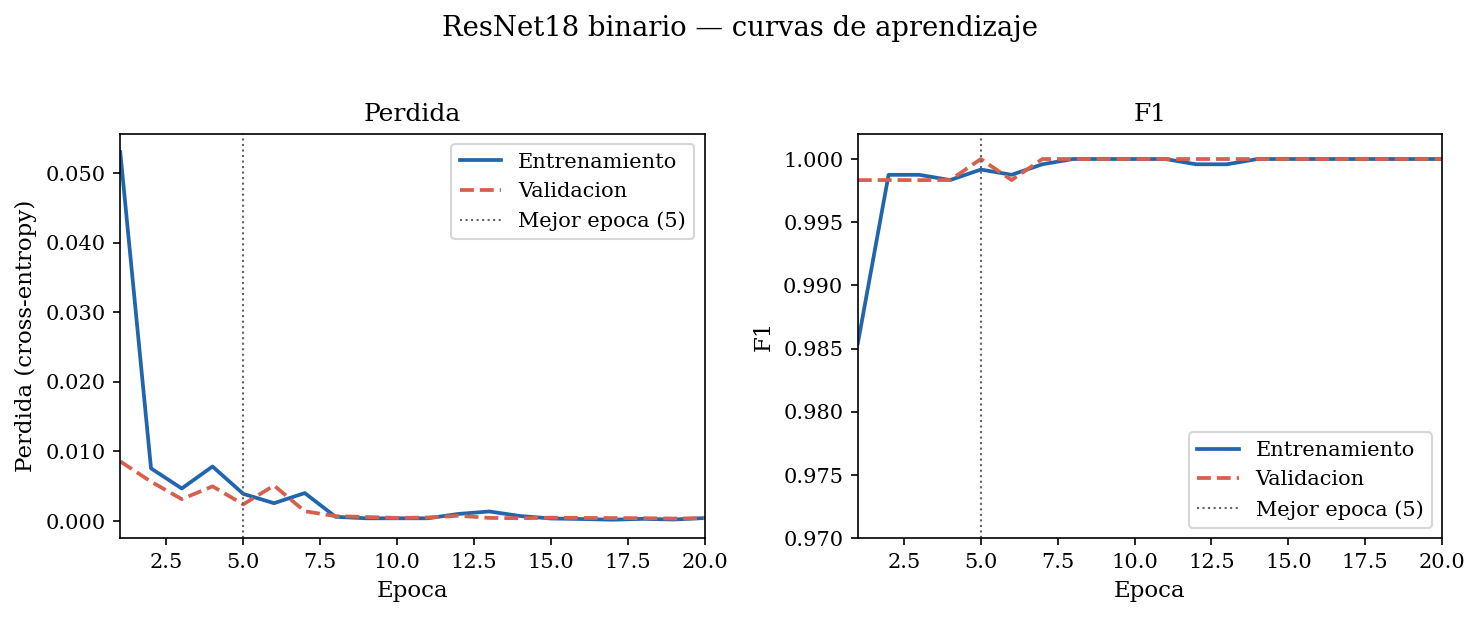
\includegraphics[width=0.85\textwidth]{figuras/resultados/resnet18_binary_curvas.png}
    \caption{Evolución de la pérdida y el F1~macro en entrenamiento y validación del clasificador ResNet18 binario a lo largo de las veinte épocas. La convergencia es extremadamente rápida: en menos de cinco épocas el F1 de validación alcanza \num{1,000}. La pérdida de validación se sitúa consistentemente por debajo de la de entrenamiento, lo que es habitual cuando el \emph{dropout} penaliza la pasada de entrenamiento pero no la de validación. No se observa sobreajuste en las curvas.}
    \label{fig:resnet18_binary_curvas}
\end{figure}

El modelo converge en menos de cinco épocas. La \cref{tab:p1_curva} detalla los valores de las primeras ocho épocas. En las épocas~1 a~4 el clasificador comete exactamente un error sobre las \num{450}~muestras de validación (F1~val = 0,998), que corresponde a una única muestra de interferencia con ráfagas Bluetooth morfológicamente próximas a OcuSync. Este error desaparece en la época~5, a partir de la cual el F1~de validación alcanza \num{1,000} con oscilaciones mínimas (una vuelta a \num{0,998} en la época~6, seguida de estabilización en \num{1,000} a partir de la época~7).

\begin{table}[htbp]
\centering
\caption{Pérdida y F1~macro durante las primeras ocho épocas del clasificador ResNet18 binario.}
\label{tab:p1_curva}
\begin{tabular}{ccccc}
\toprule
\textbf{Época} & \textbf{Loss train} & \textbf{F1 train} & \textbf{Loss val} & \textbf{F1 val} \\
\midrule
1 & 0,0530 & 0,985 & 0,0085 & 0,998 \\
2 & 0,0075 & 0,999 & 0,0056 & 0,998 \\
3 & 0,0046 & 0,999 & 0,0031 & 0,998 \\
4 & 0,0078 & 0,998 & 0,0050 & 0,998 \\
5 & 0,0039 & 0,999 & 0,0024 & 1,000 \\
6 & 0,0025 & 0,999 & 0,0051 & 0,998 \\
7 & 0,0040 & 1,000 & 0,0014 & 1,000 \\
8 & 0,0006 & 1,000 & 0,0007 & 1,000 \\
\bottomrule
\end{tabular}
\end{table}

El \emph{checkpoint} de la época~5 se evalúa sobre el conjunto de prueba con los resultados de la \cref{tab:p1_test}. La clasificación es perfecta en todas las métricas: las \num{300}~muestras de la clase \emph{drone} y las \num{300}~de \emph{interference} se asignan correctamente, sin errores en ninguna dirección.

\begin{table}[htbp]
\centering
\caption{Resultados del clasificador ResNet18 binario sobre el conjunto de prueba (\num{600}~espectrogramas, \emph{checkpoint} época~5).}
\label{tab:p1_test}
\begin{tabular}{lc}
\toprule
\textbf{Métrica} & \textbf{Valor} \\
\midrule
Exactitud         & 1,000 \\
F1~macro          & 1,000 \\
Precisión macro   & 1,000 \\
Recall macro      & 1,000 \\
\bottomrule
\end{tabular}
\end{table}

\subsubsection{¿Dónde mira la red? Análisis GradCAM}
\label{sec:p1_gradcam}

La clasificación perfecta de la \cref{tab:p1_test} no informa de \emph{por qué} la red decide como decide. Una exactitud del \SI{100}{\percent} es compatible tanto con un modelo que aprende la morfología de las ráfagas FHSS como con un modelo que explota cualquier diferencia sistemática entre las dos clases ajena a la señal. Para discriminar entre ambas hipótesis se aplica GradCAM sobre muestras del conjunto de prueba.

GradCAM calcula el gradiente de la puntuación de la clase respecto a los mapas de activación de la última capa convolucional (\texttt{layer4} de la ResNet18) y los combina ponderadamente para producir un mapa de calor sobre la imagen de entrada. Las regiones con mayor activación son las que más contribuyen a la predicción: si el clasificador resolviera la decisión a partir de la firma OcuSync, el mapa de calor debería concentrarse sobre las ráfagas FHSS verticales y diferir claramente entre una captura de dron y una de interferencia.

La \cref{fig:resnet18_gradcam_drone} muestra el resultado para cuatro espectrogramas de la clase \emph{drone}, y la \cref{fig:resnet18_gradcam_interference} para cuatro de la clase \emph{interference}. En ambas figuras la columna izquierda es la entrada tras la normalización frecuencial y la derecha el mapa GradCAM de la clase verdadera de cada fila superpuesto sobre esa misma entrada.

\begin{figure}[htbp]
    \centering
    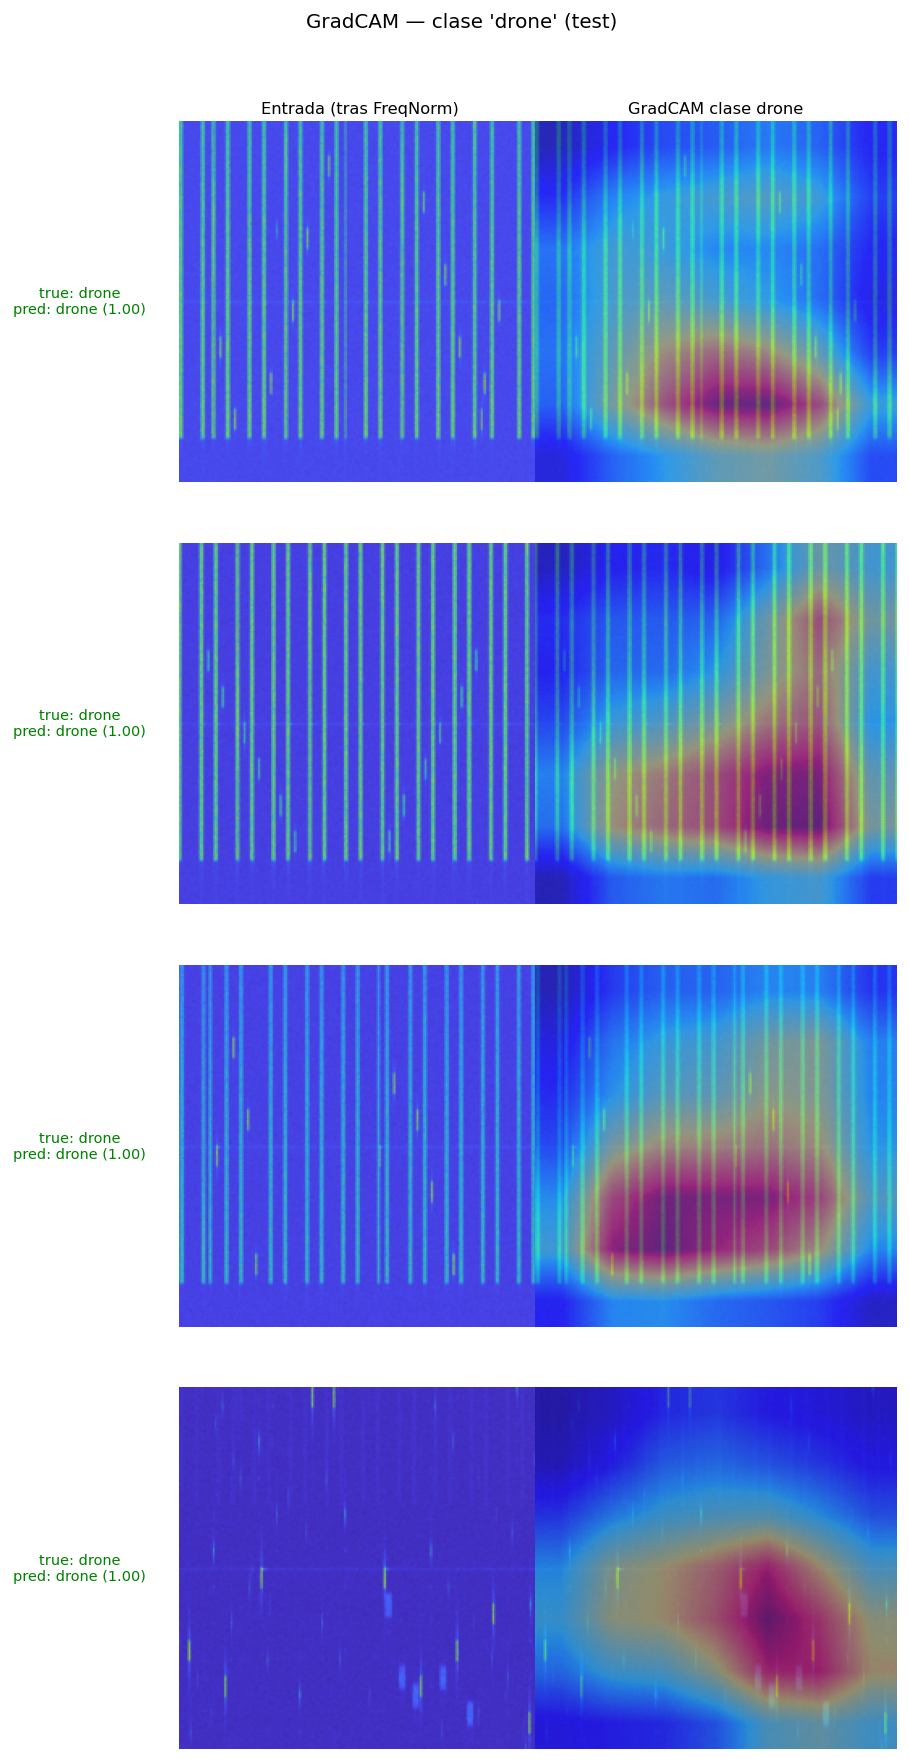
\includegraphics[width=0.80\textwidth]{figuras/resultados/resnet18_gradcam_drone.png}
    \caption{GradCAM del clasificador ResNet18 binario sobre cuatro espectrogramas de la clase \emph{drone}. Izquierda: entrada tras \texttt{FrequencyNormalize}, con las ráfagas FHSS verticales de OcuSync claramente visibles. Derecha: mapa de calor de la clase \emph{drone}. La activación es una mancha difusa y compacta situada en la región central-inferior de la imagen, que no sigue la estructura vertical de las ráfagas ni se extiende a las que aparecen en los bordes. El máximo de activación coincide con el centro geométrico del espectrograma, no con ninguna ráfaga concreta.}
    \label{fig:resnet18_gradcam_drone}
\end{figure}

\begin{figure}[htbp]
    \centering
    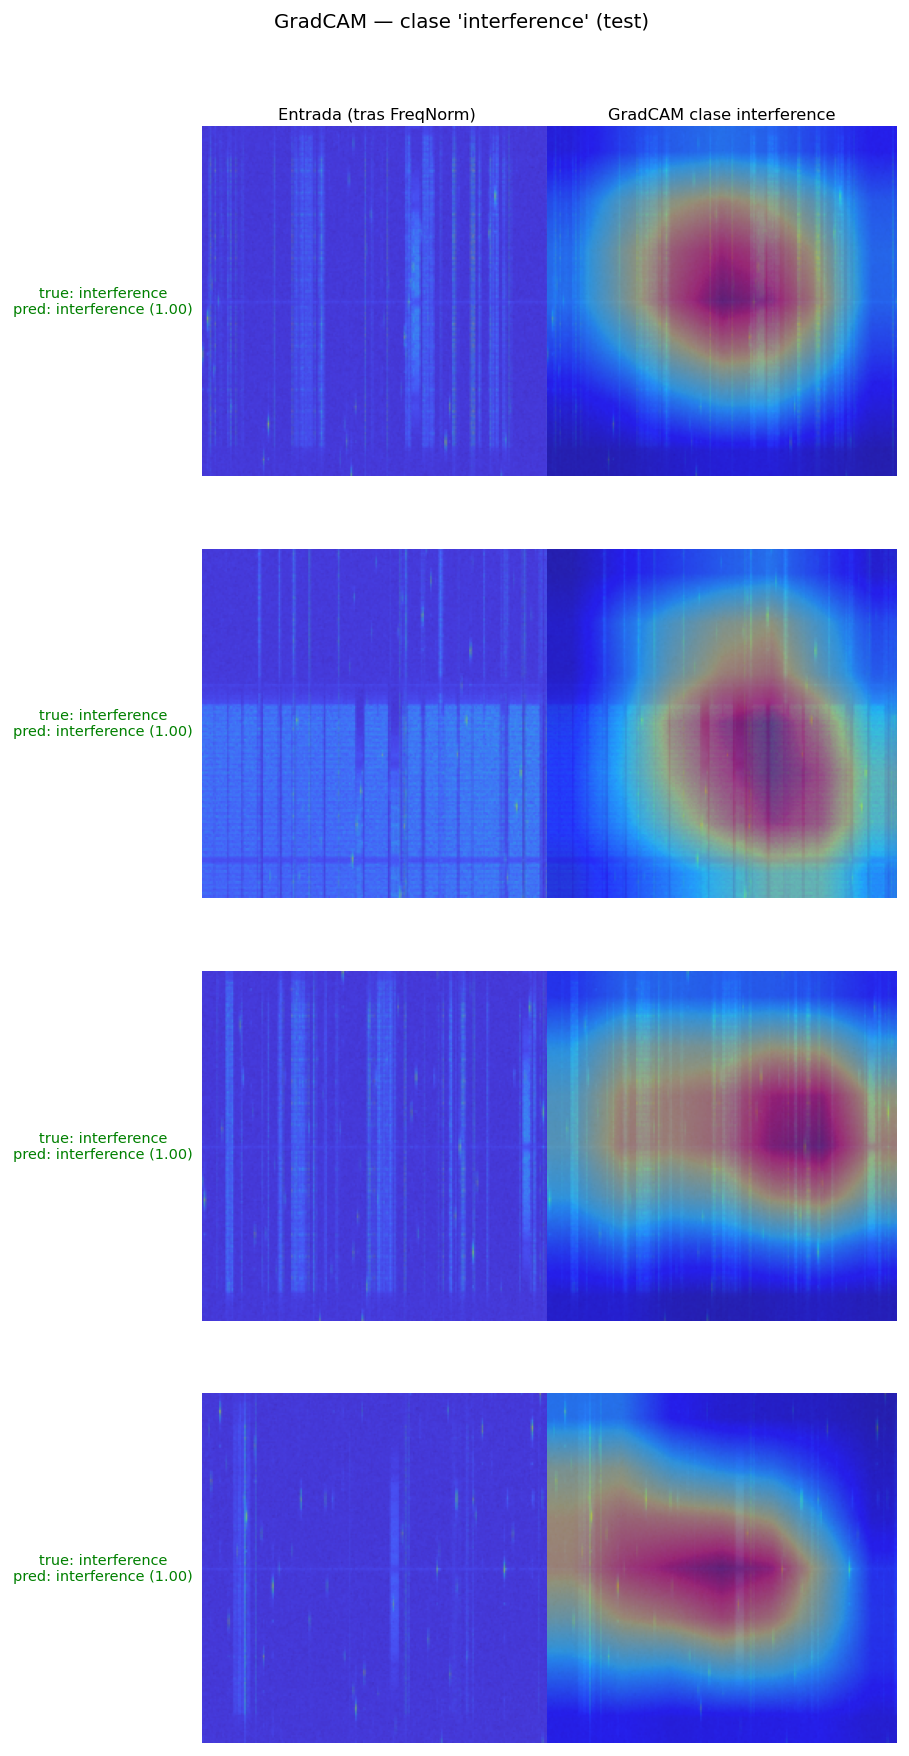
\includegraphics[width=0.80\textwidth]{figuras/resultados/resnet18_gradcam_interference.png}
    \caption{GradCAM del clasificador ResNet18 binario sobre cuatro espectrogramas de la clase \emph{interference}. Izquierda: entrada tras \texttt{FrequencyNormalize}, con señales WiFi y Bluetooth dispersas y de menor energía. Derecha: mapa de calor de la clase \emph{interference}. La activación es de nuevo una mancha difusa centrada, prácticamente idéntica en forma y posición a la de la clase \emph{drone} de la \cref{fig:resnet18_gradcam_drone}, pese a que la imagen de entrada es completamente distinta.}
    \label{fig:resnet18_gradcam_interference}
\end{figure}

El resultado es revelador y contrario a lo que cabría esperar de un modelo que hubiese aprendido la firma RF. En las capturas de dron (\cref{fig:resnet18_gradcam_drone}) la activación no recae sobre las ráfagas FHSS: forma una mancha difusa y suave en la región central-inferior que ignora la estructura vertical periódica de OcuSync y deja fuera las ráfagas de los bordes. En las capturas de interferencia (\cref{fig:resnet18_gradcam_interference}) el mapa de calor es esencialmente el mismo --- una mancha central de forma y posición casi indistinguibles --- a pesar de que el contenido de las dos imágenes no tiene nada en común.

La conclusión es directa: \textbf{los dos mapas de calor son prácticamente iguales entre clases}. Si la red estuviera discriminando por la morfología de la señal, el GradCAM de cada clase debería localizarse sobre estructuras distintas; en cambio, ambas predicciones se sustentan sobre la misma región central genérica de la imagen. GradCAM no consigue señalar ninguna evidencia local, específica de clase, que justifique la decisión. El clasificador alcanza F1\,=\,\num{1,000}, pero su atención no está anclada a la firma OcuSync, sino a un atributo difuso y global del espectrograma.

\subsection{Discusión}
\label{sec:p1_discusion}

El experimento P1 deja una conclusión de doble filo. Por un lado, confirma que las dos clases son perfectamente separables con la información del espectrograma completo: la exactitud del \SI{100}{\percent} demuestra que existe \emph{alguna} característica que distingue sin error una captura con dron de una de interferencia. Por otro lado, el análisis GradCAM demuestra que \textbf{esa característica no es la morfología de las ráfagas FHSS}. Una exactitud perfecta acompañada de mapas de saliencia difusos e idénticos entre clases es la huella típica de un clasificador que ha aprendido un \emph{atajo}: un atributo global de la captura --- nivel medio de potencia, brillo de fondo, condiciones del entorno de grabación --- correlacionado con la etiqueta pero ajeno a la señal del dron.

Este hallazgo es precisamente lo que invalida la clasificación global como criterio de detección, por tres motivos que se refuerzan entre sí.

El primero es la falta de auditabilidad. Un sistema de vigilancia debe poder justificar cada alarma señalando la evidencia concreta que la motiva. Un clasificador cuyo GradCAM apunta a una mancha central inespecífica no ofrece ninguna justificación verificable: no se puede saber qué parte de la señal ha disparado la decisión, ni distinguir una detección legítima de una casualidad estadística del conjunto de datos.

El segundo es la fragilidad ante el cambio de dominio. Si la decisión se apoya en un atributo global del entorno de captura y no en la firma RF, basta con que cambien las condiciones de grabación --- otra ganancia, otro recinto, exterior en lugar de interior --- para que la correlación aprendida se rompa y el rendimiento se desplome, aun cuando la señal del dron sea idéntica. La poca variabilidad intraclase del dataset~v3 (un único modelo de dron, un único entorno interior) hace que el atajo sea especialmente fácil de aprender y, por tanto, especialmente engañoso: el F1\,=\,\num{1,000} mide la capacidad de separar \emph{estas} capturas, no la de reconocer la firma de un dron en general.

El tercero es la ausencia de localización y de aprendizaje multietiqueta. El clasificador emite una única etiqueta para toda la imagen, de modo que no puede indicar en qué región del espectrograma está la señal ni representar la coexistencia de dron e interferencia en la misma ventana temporal, una situación habitual en un escenario real.

En conjunto, P1 demuestra que la pregunta «¿es la firma OcuSync separable?» tiene respuesta afirmativa, pero que un clasificador global no es la herramienta adecuada para responderla de forma fiable: acierta por las razones equivocadas. Estas limitaciones motivan directamente el experimento P2 --- reformular la tarea como detección de objetos ---, que obliga al modelo a justificar cada predicción con la región concreta del espectrograma que la soporta y, con ello, a aprender la morfología local de las ráfagas en lugar de un atajo contextual.
